% !TEX encoding = UTF-8 Unicode
\documentclass[a4paper]{article}

\usepackage{color}
\usepackage{url}
\usepackage[T2A]{fontenc} % enable Cyrillic fonts
\usepackage[utf8]{inputenc} % make weird characters work
\usepackage{graphicx}
\graphicspath{ {./images/} }
\usepackage{amsfonts}
\usepackage[english,serbian]{babel}
%\usepackage[english,serbianc]{babel} %ukljuciti babel sa ovim opcijama, umesto gornjim, ukoliko se koristi cirilica

\usepackage[unicode]{hyperref}
\hypersetup{colorlinks,citecolor=green,filecolor=green,linkcolor=blue,urlcolor=blue}

\usepackage{listings}
\usepackage{mathtools}
\usepackage{dirtytalk}
\usepackage{epigraph}


%\newtheorem{primer}{Пример}[section] %ćirilični primer
\newtheorem{primer}{Primer}[section]

\definecolor{mygreen}{rgb}{0,0.6,0}
\definecolor{mygray}{rgb}{0.5,0.5,0.5}
\definecolor{mymauve}{rgb}{0.58,0,0.82}

\lstset{ 
  backgroundcolor=\color{white},   % choose the background color; you must add \usepackage{color} or \usepackage{xcolor}; should come as last argument
  basicstyle=\scriptsize\ttfamily,        % the size of the fonts that are used for the code
  breakatwhitespace=false,         % sets if automatic breaks should only happen at whitespace
  breaklines=true,                 % sets automatic line breaking
  captionpos=b,                    % sets the caption-position to bottom
  commentstyle=\color{mygreen},    % comment style
  deletekeywords={...},            % if you want to delete keywords from the given language
  escapeinside={\%*}{*)},          % if you want to add LaTeX within your code
  extendedchars=true,              % lets you use non-ASCII characters; for 8-bits encodings only, does not work with UTF-8
  firstnumber=1000,                % start line enumeration with line 1000
  frame=single,	                   % adds a frame around the code
  keepspaces=true,                 % keeps spaces in text, useful for keeping indentation of code (possibly needs columns=flexible)
  keywordstyle=\color{blue},       % keyword style
  language=Python,                 % the language of the code
  morekeywords={*,...},            % if you want to add more keywords to the set
  numbers=left,                    % where to put the line-numbers; possible values are (none, left, right)
  numbersep=5pt,                   % how far the line-numbers are from the code
  numberstyle=\tiny\color{mygray}, % the style that is used for the line-numbers
  rulecolor=\color{black},         % if not set, the frame-color may be changed on line-breaks within not-black text (e.g. comments (green here))
  showspaces=false,                % show spaces everywhere adding particular underscores; it overrides 'showstringspaces'
  showstringspaces=false,          % underline spaces within strings only
  showtabs=false,                  % show tabs within strings adding particular underscores
  stepnumber=2,                    % the step between two line-numbers. If it's 1, each line will be numbered
  stringstyle=\color{mymauve},     % string literal style
  tabsize=2,	                   % sets default tabsize to 2 spaces
  title=\lstname                   % show the filename of files included with \lstinputlisting; also try caption instead of title
}

\begin{document}

\title{Optimizacija rojem čestica\\ \small{Seminarski rad u okviru kursa\\Metodologija stručnog i naučnog rada\\ Matematički fakultet}}

\author{Nevena Soldat, Milena Kurtić, Tijana Živković, Ana Miloradović\protect\\
\small{\texttt{nevenasoldat@gmail.com,}  \texttt{mimikurtic67@gmail.com,}} \\ \small{\texttt{tijanazivkovic6@gmail.com,} \texttt{ana.miloradovic7@gmail.com}}}

%\date{9.~april 2015.}

\maketitle

\abstract{ Kennedy i Eberhart (2001): \\
\say{... gledamo u paradigmu koja je u svom začeću, puna potencijala i novih ideja i novih perspektiva... Istraživači u mnogim zemljama eksperimentišu sa rojevima čestica... Mnoga pitanja koja su postavljena još uvek nisu dobila dobar odgovor \cite{poli2007particle}}

U ovom radu predstavljeni su osnovni koncepti optimizacione tehnike zasnovane na roju čestica. Opisani su glavni algoritmi, značaj i varijacije parametara, primene ove tehnike kao i različite populacione strukture čijim menjanjem, kao i menjanjem parametara, možemo da podešavamo i prilagođavamo ovu populacionu tehniku različitim problemima. 
}

\tableofcontents

\newpage

\section{Uvod}
\label{sec:uvod}

Inteligencija rojeva predstavlja jednu od paradigmi Računarske Inteligencije (eng. Computational Intelligence - CI). Jedinke u okviru grupe (roja) dele prikupljene informacije u zajedničkom cilju da reše neki problem, koje se propagiraju kroz celu grupu tako da se problem rešava mnogo efikasnije nego što bi to mogla pojedinačna jedinka.

Optimizacija rojem čestica (eng. Particle Swarm Optimization - PSO) je stohastička optimizaciona tehnika zasnovana na veoma inteligentnom kolektivnom ponašanju nekih organizama kao što su insekti, ptice i ribe.

\subsection{Kratak istorijat}
Prvi i dosta značajan doprinos u polju inteligencije rojeva imao je južnoafrički pesnik Eugene Marais\footnote{Eugène Nielen Marais (9. januar 1871 – 29. mart 1936) je bio južnoafrički advokat, naturalista, pesnik i pisac.} koji je proučavao socijalno ponašanje kako majmuna, tako i mrava. Posle njega, ranih 1990-ih godina, Marco Dorigo\footnote{Marco Dorigo (26. avgust 1961) - italijanski istraživač na polju veštačke inteligencije} modeluje ponašanje kolonija mrava. Zatim, 1995, Eberhart\footnote{Russell C. Eberhart (1950) - američki elektroinženjer} i Kennedy\footnote{James Kennedy (5. novembar 1950) - američki psiholog} razvijaju algoritam optimizacije rojem čestica, na osnovu posmatranog jata ptica.

 Algoritam optimizacije rojem čestica otkriven je sasvim slučajno, pri pokušaju da se na računaru simulira kretanje jata ptica. Prvobitna namera bila je da se grafički prikaže nepredvidiva koreografija jata ptica, sa ciljem da se otkriju obrasci koji omogućavaju pticama da lete sinhronizovano, i da zadrže optimalnu formaciju pri naglim promenama pravaca. Sada je cilj kreiranje jednostavnog i efikasnog optimizacionog algoritma. Od kada je prvi put predstavljen 1995. doživeo je niz poboljšanja i nastale su brojne varijacije ovog algoritma. 


\section{Algoritam za optimizaciju rojem čestica}
Kako bismo lakše razumeli algoritam možemo zamisliti roj pčela koje lete preko polja sa cvećem \cite{10.4018/IJRSDA.2018040101}. Roj ima urođenu želju da pronađe poziciju gde je cveće najgušće raspoređeno. Takođe, pčele nemaju nikakvo znanje o polju na kom se nalaze. Tako počinju svoju pretragu u različitim smerovima. Svaka pčela pamti mesta na kojima je bila i na kojim je bilo najviše cveća, i tu informaciju može preneti komunikacijom sa ostatkom roja. Kako vreme prolazi, pčele biraju da li će se vratiti na svoje prethodno pronađene najbolje lokacije ili će ići ka lokacijama koje su dobile od ostalih pčela. One koje oklevaju će ići u oba pravca i nalaziće se negde između ciljanih lokacija, u zavisnosti od toga da li će uticaj roja biti dominantan ili ne. Povremeno pčela može da preleti preko dela polja u kom se nalazi više cveća od do sad otkrivenih lokacija. Tada će se čitav roj povlačiti ka novootkrivenoj lokaciji.
\begin{figure}[htp]
    \centering
    \includegraphics[scale=1.2]{bees.png}
    \caption{Prikaz PSO algoritma na kojem pčele traže cveće}
    \label{fig:bees}
\end{figure}
\\ \indent Na slici \ref{fig:bees}, isprekidane linije predstavljaju zamišljene putanje pčela, a strelice prikazuju dve komponente brzine - lokalno najbolju poziciju i globalno najbolju poziciju (u datom trenutku). Pčela u gornjem delu slike je pronašla globalno najbolju poziciju, dok je pčela sa leve strane pronašla lokalno najbolju poziciju. Pčela u donjem delu slike prikazuje da iako nije pronašla lokalno najbolju poziciju, ide ka globalno najboljoj poziciji. \\
\indent Na ovaj način pčele pretražuju polje tako što menjaju brzine i pravac kretanja u zavisnosti od toga da li su imale uspeha da pronađu cveće u odnosu na čitav roj. Takođe, pčele znaju da izbegavaju mesta koja nisu imala puno cveća. Na kraju će pretražiti celo polje, i nalaziće se iznad mesta na kojem je najveća gustina cveća.

\subsection{Originalni PSO}
Algoritam za optimizaciju rojem čestica sadrži jedinke koje se kreću kroz višedimenzioni prostor pretrage, a pozicije jedinki se menjaju u skladu sa sopstvenim iskustvom, kao i sa iskustvom susednih jedinki. Svaka od tih čestica predstavlja jedno moguće rešenje.
Neka je $x_i(t)$ pozicija čestice \textit{i} u prostoru pretrage u trenutku \textit{t}. Pozicija čestice se menja dodavanjem brzine, $v_i(t)$ na trenutnu poziciju. \[x_i(t+1) = x_i(t) + v_i(t+1) \]
Njihovo kretanje se usmerava imajući u vidu njihovu trenutnu poziciju, njihovu do sada najbolju poziciju, kao i do sada najbolju poziciju čitavog roja. Kognitivna komponenta algoritma predstavlja tendenciju vraćanja u lično najbolje rešenje, dok socijalna komponenta predstavlja tendenciju ka globalno najboljem rešenju. Brzina se računa kao: \[ v_i(t+1) = v_i(t) + c_1r_1(p_i(t) - x_i(t)) + c_2r_2(p_g(t) - x_i(t))\]
gde $p_i(t)$ predstavlja najbolju do sada poziciju čestice \textit{i} u trenutku t, dok je $p_g(t)$ globalno najbolje rešenje (pozicija) do trenutka t. Parametri $r_1$ i $r_2$ su nasumične vrednosti izabrane iz uniformne raspodele na intervalu [0,1], i predstavljaju stohastičku komponentu algoritma. Parametri $c_1$ i $c_2$ su konstante koje predstavljaju pozitivna ubrzanja čija je uloga da skaliraju značaj kognitivne, odnosno socijalne komponente brzine. 
Pseudokod originalnog PSO algoritma: \\ \\
\textbf{Algoritam} \textit{osnovni} PSO: \\ 
Kreiraj i inicijalizuj $n_s$ - dimenzioni roj;\\
\textbf{ponavljaj} \\ 
\hspace*{5mm}\textbf{za} \textit{svaku česticu} $\textit{i} = 1,...,n_s$ \textbf{uradi} \\
\hspace*{5mm} // postavi lokalno najbolju poziciju \\
\hspace*{10mm} \textbf{ako} $f(x_i) < f(p_i)$ \textbf{onda} \\
\hspace*{15mm} $p_i = x_i;$ \\
\hspace*{10mm} \textbf{kraj} \\
\hspace*{5mm}//postavi globalno najbolju poziciju \\\
\hspace*{10mm}\textbf{ako} $f(p_i) < f(p_g)$ \textbf{onda} \\
\hspace*{15mm} $p_g = p_i;$ \\
\hspace*{10mm} \textbf{kraj} \\
\hspace*{5mm} \textbf{kraj} \\
\hspace*{5mm} \textbf{za} \textit{svaku česticu} $i = 1,...,n_s$ \textbf{uradi}\\
\hspace*{10mm} ažuriraj brzinu; \\
\hspace*{10mm} ažiriraj poziciju; \\
\hspace*{5mm} \textbf{kraj} \\
\textbf{dok} nije ispunjen zahtev za zaustavljanje; \\ \\Funkcija $f:\mathbb{R}^{n_s} \to \mathbb{R}$ je fitnes funkcija. Fitnes funkcija računa koliko je dobijeno rešenje blisko optimalnom, odnosno meri kvalitet rešenja.
\subsection{Komponente brzine PSO algoritma}
Brzina \textit{i}-te čestice ima tri komponente:\\
\begin{itemize}
    \item \textbf{Prethodna vrednost brzine}, $\textbf{v}_i(t)$, koja čuva prethodni pravac kretanja čestice. Može se reći da je ona moment koji sprečava česticu da drastično promeni pravac. 
    \item \textbf{Kognitivna komponenta}, $c_1\textbf{r}_1(\textbf{p}_i - \textbf{x}_i)$,  može se opisati kao pamćenje najbolje pozicije u kojoj se čestica do sada našla. Efekat ove komponente je tendencija čestica da se vrate na pronadjene najbolje pozicije. Kennedy i Eberhart su nazivali koginitivnu komponentu \say{nostalgija} čestice.
    \item \textbf{Socijalna komponenta}, $c_2\textbf{r}_2(\textbf{p}_g - \textbf{x}_i)$, koja meri rezultat čestice \textit{i} u odnosu na sve susedne čestice. Efekat ove komponente je tendencija čestice da se kreće ka najboljoj poziciji pronađenoj od strane susednih čestica.
\end{itemize}

\begin{figure}[htp]
    \centering
    \includegraphics[scale=1.7]{velocity.png}
    \caption{Prikaz promene brzine}
    \label{fig:velocity}
\end{figure}

U svakoj generaciji, iterativni proces čestice izgleda kao na slici \ref{fig:velocity}. Analizirajući ažuriranje brzine vidimo da je prvi deo uticaj prethodne brzine čestice. To znači da čestica veruje da je na dobrom putu i kreće se inercijalno. Drugi deo zavisi od trenutne pozicije čestice i njene najbolje pozicije do sada, odnosno od kognitivne komponente brzine. Treći deo se oslanja na udaljenost trenutne pozicije čestice i globalno najbolje pozicije u roju, odnosno na socijalnu komponentu brzine \cite{wang2018particle}. 

\subsection{Algoritmi gbest i lbest PSO}
\label{subsec:podnaslov1}

U slučaju globalno najboljeg PSO algoritma (eng. Global Best - \textit{gbest}) čestice mogu da komuniciraju sa svim ostalim česticama u roju, i na taj način ceo roj deli informaciju o najboljoj poziciji koja je pronađena (globalno najbolja pozicija). Ovaj pristup može dovesti do toga da ceo roj ostane zaglavljen u tački lokalnog minimuma, pa tako nastaju i mnoge druge topologije mreže.

Lokalno najbolji PSO (eng. Local Best - \textit{lbest}) podrazumeva da čestice dele informacije sa određenim podskupom čestica u roju (susedima). Doprinos jedinke brzini je proporcionalna razdaljini između čestice i najbolje pozicije koju su pronašli susedi. 

Zbog bolje povezanosti čestica u gbest algoritmu, on brže konvergira ka rešenju. Cena brže konvergencije je manja raznovrsnost. Kao posledica veće raznovrsnosti (što podrazumeva da je veći deo prostora pretrage pokriven), lbest PSO ima manje šanse da ostane zarobljen u lokalnom optimumu. \cite{engelbrecht2007computational}.

Razvijene su mnoge strategije na osnovu kojih se bira susedstvo, kao što je razdaljina u prostoru. Međutim, preferirano rešenje je odabir na osnovu indeksa, i za to postoje dva glavna razloga:
\begin{enumerate}
    \item Za pristupe koji podrazumevaju računanje udaljenosti između čestica, potrebno je naći Euklidsko rastojanje svih parova čestica, a to ima veliku složenost ($(n_s)^2$).
    \item Lakše je prosleđivanje informacije o dobrim rešenjima svim česticama, nezavisno od njihove lokacije u prostoru pretrage.

\end{enumerate}
Obe strategije zasnovane su na nekom socijalnom ponašanju. Zašto nije dobro birati susedstvo na osnovu udaljenosti?  Može se desiti da čestice koje su na većoj udaljenosti imaju slične osobine (kao npr. članovi jedne porodice). One nikad neće biti susedne, iako imaju sličnosti.  \cite{liu2006particle}.
    
    
\section{Osnovne varijacije}
Postoji nekoliko modifikacija osnovnog PSO algoritma \cite{rini2011particle}, a one su razvijane da bi poboljšale brzinu konvergencije i kvalitet rešenja koji ovaj algoritam nalazi.

\subsection{Smanjenje brzina}
Za efikasnost i tačnost algoritma optimizacije važno je napraviti balans između eksploracije i eksploatacije. 
$Eksploracija$ se odnosi na sposobnost algoritma pretrage da istražuje različite regione prostora pretrage da bi se pronašao dobar optimum, dok je $eksploatacija$ sposobnost  da se pretraga koncentriše oko regije koje garantuje nalaženje rešenja da bi se poboljšao kandidat rešenja. Ovo su konktradiktorni ciljevi koje treba dovesti u balans radi dobijanja dobrog optimizacionog algoritma.

Ažuriranje brzine u gorenavedenoj jednačini doprinosi veličini koraka čestice. U ranijim, osnovnim PSO algoritmima je primećeno da brzina brzo dostiže velike vrednosti, specijalno kod čestica koje su daleko od najboljih u okruženju i najboljih sopstvenih pozicija. Čestim ažuriranjem položaja jedinke polako napuštaju granice prostora pretrage, tj. divergiraju. Zato se brzine smanjuju kako bi čestice ostale u okviru granica.
\begin{equation}
    v_i(t+1) = \begin{cases}
                
            v'_i(t+1),  &  v'_i(t+1) < V_{max}\\
            V_{max},  &   v'_i(t+1) \geq V_{max}
           
             \end{cases}
\end{equation}

Velike vrednosti maksimalne brzine olakšavaju istraživanje na globalnom nivou, dok manje vrednosti podstiču lokalnu eksploataciju, obe imaju mane. Dok veoma male vrednosti mogu da povećaju broj vremenskih koraka do nalaženja optimalne vrednosti, veoma velike vrednosti brzina mogu dovesti da se sasvim propusti dobar region, ali se uz to čestice ipak brže kreću, pa treba pronaći balans.

Loša strana promene brzine leži u tome što se menja i pravac kretanja čestice, što omogućava bolju eksploraciju, ali tako optimum može da ostane nepronađen (Slika \ref{fig:smanjenje_brzina}).

\begin{figure}[htp]
    \centering
    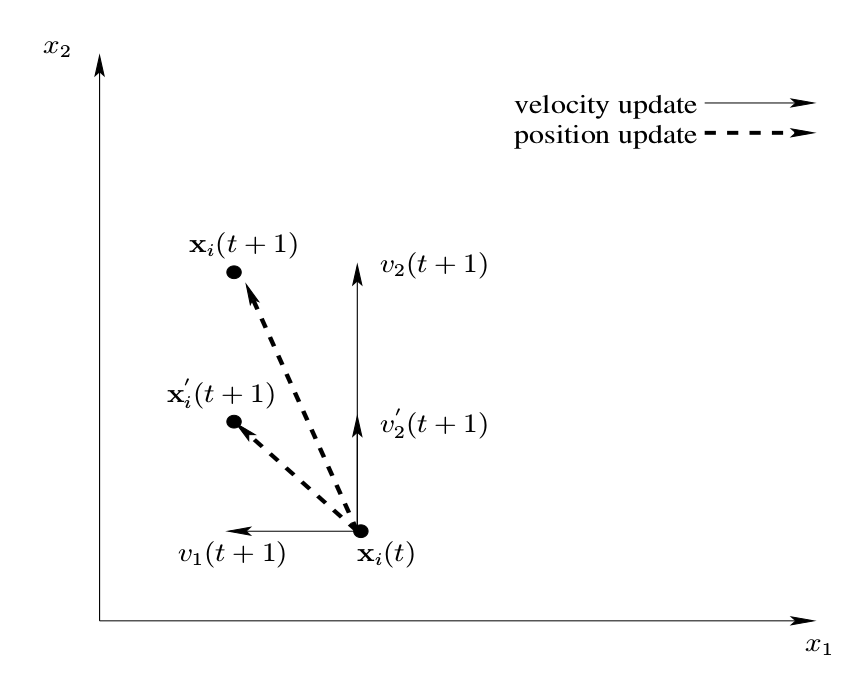
\includegraphics[scale=0.25]{slika3_1.png}
    \caption{Efekat smanjenja brzine}
    \label{fig:smanjenje_brzina}
\end{figure}

Kada su sve vrednosti jednake $V_{max}$, čestice se zaglavljuju unutar ograničene oblasti $[x_i(t)-V_{max} , x_i(t) + V_{max} ]$.  Ovaj problem se može rešiti uvođenjem inercijske težine ili smanjivanjem  $V_{max}$ vrednosti vremenom, tako što pretraga počine s velikim vrednostima i tako se pretražuje prostor, a zatim se postepeno smanjuje. Tako se ograničava globalna pretraga.

\subsection{Inercijalna težina}
Inercijalna težina uvedna je da bi se eliminisala potreba koriščenja smanjenja brzina, kao i da bi se kontrolisala sposobnost eksploracije i eksploatacije. Težina $w$ kontroliše koliko će prethodni pravac leta uticati na novu brzinu. Sada jednačina izgleda ovako:
\[v_{ij}(t+1) = wv_{ij}(t) + c_1r_{1j}(t)[y_{ij}(t) - x_{ij}(t)] + c_2r_{2j}(t)[\hat{y}_{ij}(t) - x_{ij}(t)] \]
Dolazi do promene jednačine ažuriranja brzina kod $gbest$ i $lbest$ PSO algoritama.
Kod ovog pristupa je vrednost $w$ izuzetno važna za ostvarivanje konvergencije, kao i za prethodno pomenuti balans. Razlikuju se slučaji kada je $w \geq 1$, tada se brzine povećavaju tokom vremena prema $V_{max}$ i roj divergira, dok za $w < 0$ brzine opadaju sve dok ne dostignu nulu i time se algoritam zaustavlja, a za $0 < w < 1$ čestice usporavaju, pa konvergencija zavisi od vrednosti $c_1$ i $c_2$. Tako velike vrednosti  $w$ olakšavaju eksploraciju, dok male vrednosti podstiču loakalnu eksploataciju. 
Kao i kod $V_{max}$, i ovaj pristup zavisi od samog problema. Time se u početnim koracima dozvoljava da čestice istražuju, a zatim počinju da favorizuju određene delove područja kako vreme odmiče.
Vrednost $w$ se mora birati zajedno sa vrednostima $c_1$ i $c_2$ (konstante ubrzanja).

\subsection{Koeficijent suženja}
Clerc\footnote{Maurice Clerc (rođen 1972.) diplomirani je matematičar, član Francuskog udruženja za veštačku inteligenciju i internet društva} je razvio pristup sličan inerciji težina, gde su brzine ograničene konstantom $\chi$ koji se naziva koeficijentom suženja. Jednačina sada izgleda ovako:
\[v_{ij} (t + 1) = \chi[v_{ij} (t) + \phi_1 (y_{ij} (t) - x_{ij} (t)) + \phi_2 (\hat{y}_j (t) - x_{ij} (t))]\]
gde je $$\chi = \frac{2k}{|2-\phi-\sqrt{\phi(\phi-4)}|},$$sa $\phi = \phi_1 +  \phi_2 , \phi_1 = c_1r_1$ i $\phi_2 = c_2r_2$.
Jednačina se primenjuje pod ograničenjima gde je $\phi \geq 4$ i $k$ $\in [0, 1]$
Ovaj pristup napravljen je kao prirodan, dinamički način da se osigura konvergencija ka stabilnoj tački.
Parametar $k$ u jednačini kontroliše sposobnost eksploracije i eksploatacije, za $k \approx 0$ se postiže brza konvergencija uz lokalnu eksploataciju, dok za  $k \approx 1$ sporo konvergira, sa visokim stepenom eksploracije. $k$ se obično postavlja na konstantnu vrednost.

Razlika između pristupa smanjenja brzina i koeficijenta suženja je ta da smanjenje brzina nije neophodno za model suženja. Model suženja garantuje konvergenciju pod datim ograničenjima i kod njega svaka promena smera čestica mora se izvršiti preko $\phi_1$ i $\phi_2$.

\subsection{Modeli brzina}
Modeli se razlikuju u komponentama koje su uključene u jednačinu brzine i u tome kako se utvrđuju najbolji položaji. Neki od njih su:
\begin{itemize}
    \item \textbf{Kognitivni model}, kognitivni model isključuje socijalnu komponentu iz jednačine, ilustruje stohastičku tendenciju  da se čestice vraćaju u svoju najbolju poziciju i može se uporediti sa nostalgijom. Ovaj model je sporiji, potrebno je više iteracija da bi se dostiglo dobro rešenje, a, takođe, ne uspeva kada je malo smanjenje brzina i koeficijent ubrzanja\footnote{Loše performanse ovog modela potvrđene su od strane Carlisle-a and Dozier-a u \textit{Adapting Particle Swarm Optimization to Dynamic Environments. In Proceedings of the International Conference on Artificial Intelligence, pages 429–434, 2000.}}.
    \item \textbf{Socijalni model}, socijalni model isključuje kognitivnu komponentu iz jednačine: $v_{ij} (t + 1) = v_{ij} (t) + c_2r_{2j} (t)(\hat{y}_j (t) - x_{ij} (t))$ u $gbest$ PSO algoritmu. Kod ovog modela sve čestice idu ka najboljem položaju svog okruženja. Ovaj model se pokazao bržim od originalnog i kognitivnog modela, što takođe potvrđuju maločas pomenuti rezultati Carlisle-a and Dozier-a.
    \item \textbf{Model u kojoj sama čestica neće sebe izabrati za najbolju}, kod ovog modela koji je sličan socijalnom, najbolje rešenje iz okruženja se bira isključivo iz suseda čestica. On se pokazao bržim od socijalnog modela u čak nekoliko problema\footnote{potvrđeni na istin način kao i performanse prva dva modela}.
\end{itemize}

\section{Primene}
Postoje različiti načini primene PSO algoritma. Neki od njih obuhvataju širi opseg specifičnih primena dok drugi podrazumevaju primenu na jasno definisan problem \cite{eberhart2001swarm}.
Neke od primena su sledeće:
\begin{itemize}
    \item U dizajnu antena – kontrola i dizajn faznih polja, dizajniranje i modeliranje širokopojasnih antena, ispravljanje grešaka u polju, dizajniranje ugradbenih antena…
    \item U biomedicini - u svrhu detekcije Parkinsonove bolesti na temelju drhtavice, optimizacije biomehaničkog ljudskog pokreta, klasifikacije raka i predviđanja ostatka života, dizajniranje lekova.
    \item Za dizajniranju bluetooth mreža, usmeravanje, za izgradnju radarskih mreža.
    \item Kombinatorni problemi- rešavanje problema trgovačkog putnika, optimizacija puta…
    \item U kombinaciji s neuronskim mrežamama, PSO se koristi za inverziju neuronskih mreža, kontrolu neuronskih mreža za nelinearne procese,  kontrolu mobilnih neuronskih mreža, izgradnju neuronskih kontrolora.
    \item Koristi se u funkciji predviđanja kvaliteta i klasifikacije vode, u ekološkim modelima, meteorološkim predviđanjima.
   
     
   
\end{itemize}

\subsection{Primer rešavanja problema rekonfiguracije i planiranja distributivne mreže}
\vspace{5mm} 


Topologije distributivnih mreža su dugi niz godina bile sa smanjenim mogućnostima promene strukture, zbog niskog stepena automatizacije i ograničenja daljinskog upravljanja. 
Problem određivanja optimalne konfiguracije distributivne mreže je kompleksan, kombinatoran, nelinearan, diskretan za čije rešavanje su idealne \textbf{metaheurističke} metode koje koriste modele zasnovane na prirodnim procesima među koje spada i \textbf{optimizacija rojem čestica}.

\textbf{Cilj} rekonfiguracije i planiranja distributivnog sistema je optimizacija ukupnih troškova elektroenergetske kompanije da opslužuje potrošačke zahteve – opterećenja koji obično rastu sa vremenom.\\

Za rešavanje ovog problema koristi se metaheuristička metoda zasnovana na optimizaciji rojem čestica sa ciljem minimizacije ukupnih gubitaka aktivne snage u mreži. 

\vspace{15mm} 

\begin{flushleft}
\textbf{Formulisanje problema:} 
\end{flushleft}

Rekonfiguracija distributivne mreže sa ciljem minimizacije ukupnih gubitaka aktivne snage u mreži prema teoriji grafova svodi se na pronalazak optimalne konfiguracije mreže, odnosno pronalazak razapinjujućeg stabla grafa za koji je optimizacioni kriterijum ispunjen. Pod razapinjujućem stablom (eng. spanning trees) podrazumevamo podgraf koji se dobija iz grafa uklanjanjem određenog broja  grana iz grafa, a da pritom graf ostane povezan sa istim brojem čvorova. 

\vspace{5mm} 

\begin{flushleft}
Faktori koji se moraju razmatrati  u optimizaciji distributivnog sistema:
\end{flushleft}

\begin{itemize}
    \item minimizacija gubitka energije,
    \item minimizacija ulaganja u nove objekte i distributivnih vodova,
    \item maksimizacija pouzdanosti sistema.
\end{itemize}

\begin{flushleft}
Povrh toga, neka ograničenja se moraju uzeti u obzir:
\end{flushleft}

\begin{itemize}
    \item kapacitet vodova,
    \item naponski nivo opterećenja u čvorovima,
    \item grafikon povezivanja,
    \item radijalnost mreže.
\end{itemize}

\vspace{5mm} 

Problem je formulisan sa dve funkcije cilja. Prva funkcija cilja odnosi se na gubitke energije. U ovoj funkciji figurišu troškovi održavanja i troškovi gubitaka kao i fiksni troškovi. Druga funkcija cilja koja se koristi je vezana za pouzdanost sistema i smanjuje ukupnu neisporučenu energiju. U ovoj funkciji figurišu stope otkaza i trajanja popravke svake napojne grane. Minimizacija ovog cilja maksimizuje pouzdanost mreža.

\vspace{5mm} 

Prema \(x_{i d}^{k+1} = x_{i d}^{k} + v_{i d}^{k+1}  \) pozicija i–te čestice u d–dimenzionalnom prostoru rešenja izračunata u k+1-oj iteraciji u opštem slučaju nije celi broj, što znači da se PSO algoritam ne može primenjivati za rešavanje diskretnih optimizacionih problema. U tu svrhu 1997. godine Eberhart i Kennedy predstavili su binarnu verziju PSO algoritma, koja predstavlja modifikaciju PSO algoritma za rešavanje diskretnih optimizacionih problema. Modifikacija se ogleda kroz normalizaciju brzine čestice na datoj poziciji u intervalu [0, 1].

\vspace{5mm} 

\begin{flushleft}
\textbf{Kodiranje čestica:} 
\end{flushleft}

Šema kodiranja čestica kodira topologiju mreže, odnosno, transformatorske stanice i putanje fidera. Najčešće korišćeno kodiranje je direktno međutim slabost takvog pristupa je potencijalno dobijanje upetljanih mreža. Da bi se to izbeglo, koristi se hibridni pristup direktnog i indirektnog kodiranja, gde čestice sadrže dva segmenta.

\vspace{5mm} 

\begin{itemize}
\item \textbf{Segment fidera} – Sastoji se od podsegmenta “pristrasnosti” čvora vrednosti $\rho$,  $\rho \in (-1,1)$, odnosno, indirektna informacija koja dekodiranjem daje mrežnu topologiju i drugi podsegment sadrži broj fidera (\(N_{Fi}\) za transformatorske podstanice i) za svaku podstanicu, što je direktna informacija.

\item \textbf{Segment trafostanica} – Sadrži direktne informacije o lokacijama svake transformatorske stanice  (\(X_{i}\) i \(Y_{i}\), koordinate transformatorskih stanica u dvodimenzionoj ravni).
\end{itemize}

\begin{figure}[htp]
    \centering
    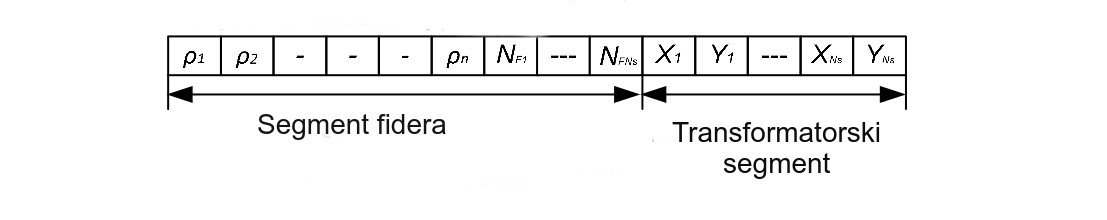
\includegraphics[scale=0.3]{foto4.jpg}
    \caption{Šema kodiranja}
    \label{fig:sema_kodiranja}
\end{figure}

\begin{flushleft}
\textbf{Šema dekodiranja:} 
\end{flushleft}

U ovom pristupu čvorovi su uzastopno izabrani i dodati na terminalni čvor rastućom putanjom na osnovu minimalne vrednosti proizvoda troškova grane i vrednosti “pristrasnosti” čvora. Troškovi grane se uzimaju kao udaljenosti između njegovih početnih i krajnjih čvorova. Po predloženoj šemi, dobija se radijalna mreža i generišu se bočne grane u odnosu na glavne grane. Osim toga, u realnoj distributivnoj mreži, razumno je da se ograniči povezivanje čvora sa samo nekoliko susednih čvorova. Za tu svrhu formirana je matrica povezivanja M, dimenzije nxn, gde je n broj čvorova. Ako je dozvoljena veza između čvorova i i j, onda je M(i,j) =1, inače  M(i,j) =0. Moguća povezanost čvora postoji sa fiksnim brojem svojih najbližih susednih čvorova \cite{inproceedings}.\\
\\ 
\textbf{Pseudokod:} \\ 
\textbf{Početak:} /*Inicijalizacija - podešavanje veličine populacije i maksimalnog broja iteracija $k_{max}$ */ \\
\hspace*{5mm}k = 0; \\
\hspace*{5mm}$s^k = s_{i}^0;$  /*Generisanje početne tačke pretrage za celu populaciju po predloženoj šemi kodiranja */ \\
\hspace*{5mm}$v^k = v_{i}^0;$  /*Generisanje početne brzine pretrage za celu populaciju po predloženoj šemi kodiranja */ \\
\hspace*{5mm}Dekodiranje svih čestica; /*Po predloženoj šemi dekodiranja*/ \\
\hspace*{5mm}Oceniti f(k); /* Izračunati vrednosti funkcije cilja svake čestice u tekućoj populaciji k*/ \\
\textbf{Ponavljati:}/*Globalna iteracija, k*/ \\
\hspace*{5mm}$v_{i}^k+1 = wv_{i}^k + c_{1}rand_{1} x (pbest_{i} - s_{i}^k) + c_{2}rand_{2} x (gbest_{i} - s_{i}^k);$ /*Ažuriraj brzinu za sve čestice */ \\
\hspace*{5mm}$s_{i}^{k+1} = s_{i}^k + v_{i}^{k+1};$ /*Ažuriraj poziciju za sve čestice*/ \\
\hspace*{5mm}Dekodiranje svih čestica; \\
\hspace*{5mm}Oceniti f(k); /* Izračunati vrednost funkcije cilja svake čestice u tekućoj populaciji k*/ \\
\hspace*{5mm}\textbf{If} f(k)>pbest(k) \textbf{Then} pbest(k+1)=f(k) /*Prihvatiti funkciju cilja f(k) čestice kao pbest(k+1) za tu česticu*/ \\
\hspace*{5mm}\textbf{If} pbest(k)>gbest(k) \textbf{Then} gbest(k+1)=pbest(k) i pamti k-tu česticu  /*Prihvatiti pbest(k) kao gbest(k+1) i sačuvaj k-tu česticu kao najbolju*/ \\
\hspace*{5mm}$k = k+1;$ \\
\textbf{Dok} nije ispunjen zahtev za zaustavljanje; /*$k > k_{max}$  */ \\
\textbf{Izlaz:} Najbolje nađeno rešenje \\

\section{Topologije uticaja}


Na PSO direktno utiče raznolikost populacije kao i socijalna interakcija među česticama. Stoga, dizajniranje razlicitih struktura populacije predstavlja bitnu tačku istraživanja kako bi se došlo do što boljih performansi.

Čestice u roju uče jedne od drugih tako što razmenjuju informacije o uspešnosti svake čestice i na osnovu dobijenih saznanja postaju više slične svojim boljim susedima. Veći utcaj na čestice imaće sused koji je više uspešan od suseda koji je manje uspešan. Kako se informacije kreću unutar određene strukture populacije govori nam stepen povezanosti čestica, broj klastera i najmanja razdaljina između čestica. Velika povezanost čestica utiče na brzo širenje informacija, što u pogledu optimizacije dovodi do brže konvergencije ka rešenju po cenu zaglavljivanja u lokalnom minimumu. Suprotno, ako čestice nisu dobro povezane postojaće više klastera (grupacija), informacije se sporije razmenjuju i može se desiti da se ne pokrije ceo prostor pretrage.

Različite topologije uticaja su razvijane i istraživane za potrebe PSO algoritma a one koje su se najbolje pokazale su:

\begin{table}[!b]
    \centering
    \begin{tabular}{| c | c |}
    \hline
        Zvezda &  \ref{fig:ZvezdaPrstenTocak} levo  \\
    \hline    
        Prsten &  \ref{fig:ZvezdaPrstenTocak} sredina \\
    \hline
        Točak & \ref{fig:ZvezdaPrstenTocak} desno \\
    \hline
        Piramida & \ref{fig:PiramidaCetiriKlasteraFonNojman} levo \\
    \hline
        Četiri klastera & \ref{fig:PiramidaCetiriKlasteraFonNojman} sredina\\
    \hline
        Fon Nojmanova & \ref{fig:PiramidaCetiriKlasteraFonNojman} desno \\
    \hline
    \end{tabular}
    \caption{Reference}
    \label{tab:my_label}
\end{table}{c|c}


\begin{itemize}
    \item \textbf{Zvezda}: Svaka čestica komunicira sa svakom drugom česticom čime informacija o trenutno najboljoj čestici dolazi veoma brzo. Stoga, postoji mogućnost glavljenja u lokalnom minimunu. Prva implementacija PSO je koristila zvezdanu strukturu (gbest).
    \item \textbf{Prsten}: Svaka čestica komunicira sa svojih N suseda. Kada je N=2 struktura izgleda kao na slici. Razlčita susedstva se preklapaju tako da informacije teku sporije. Konvergencija je sporija i pokriva se veći prostor pretrage.
    \item \textbf{Točak}: Jedna čestica predstavlja žarište i sve informacije se prenose preko te čestice.
    \item \textbf{Piramida}: Formira se trodimenzioni žičani okvir.
    \item \textbf{Četiri klastera}: Četiri klastera povezani svaki sa svakim, dok se unutar jednog nalaze čestice povezane sa četiri suseda.
    \item \textbf{Fon Nojmanova}: Socijalna struktura gde su čestice povezane u rešetku. U određenim slučajevima pokazala se mnogo bolje nego druge strukture.
\end{itemize}
\begin{figure}[htp]
    \centering
    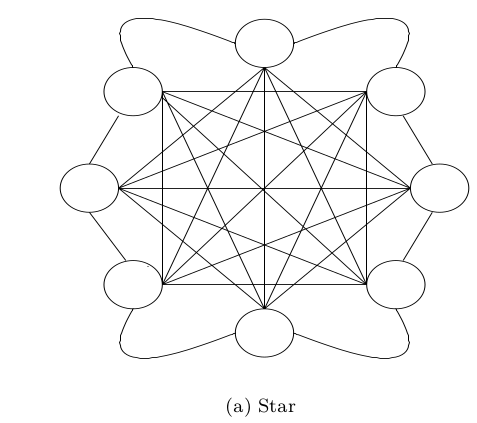
\includegraphics[scale=0.2]{Star.png}
    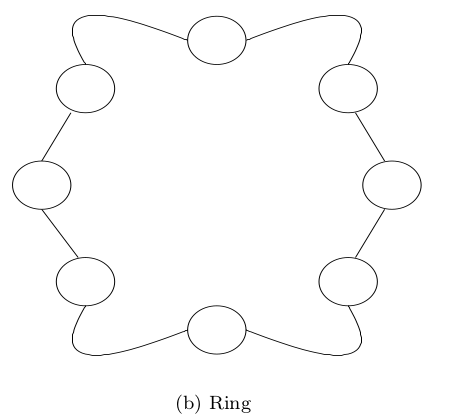
\includegraphics[scale=0.2]{Ring.png}
    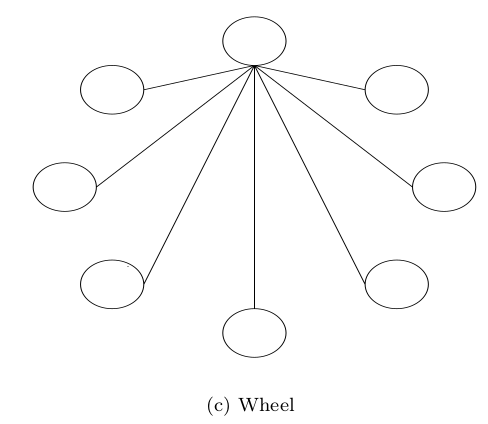
\includegraphics[scale=0.2]{Wheel.png}
    \caption{Zvezda, prsten i točak}
    \label{fig:ZvezdaPrstenTocak}
\end{figure}
\begin{figure}[htp]
    \centering
    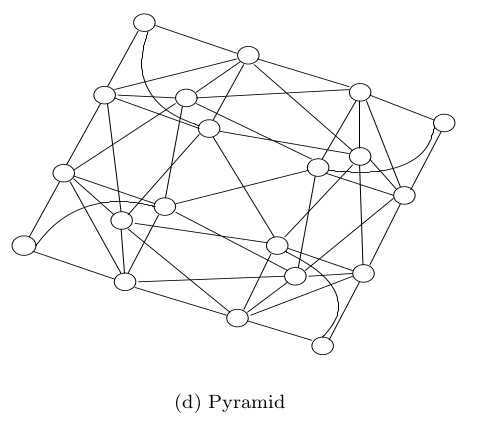
\includegraphics[scale=0.2]{Pyramid.png}
    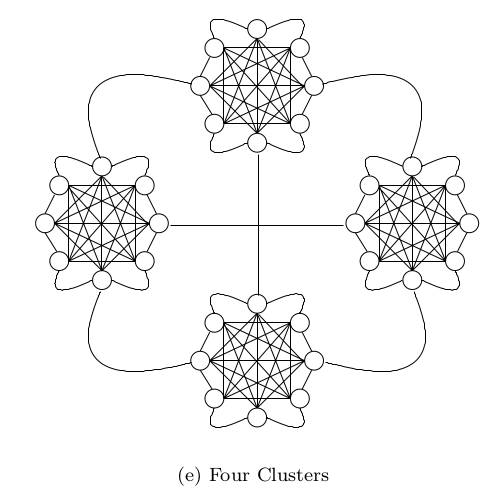
\includegraphics[scale=0.2]{FourClusters.png}
    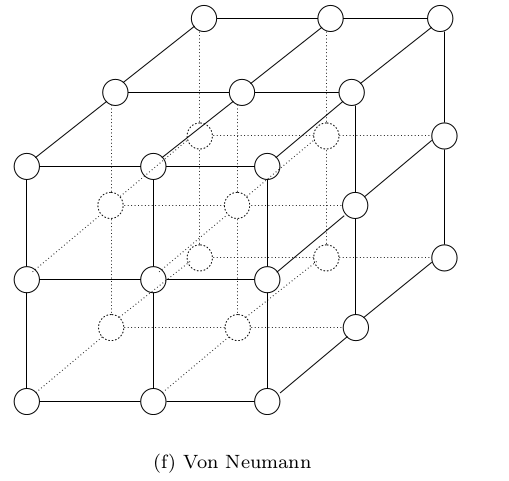
\includegraphics[scale=0.2]{VonNeumann.png}
    \caption{Piramida, četiri klastera i Fon Nojman}
    \label{fig:PiramidaCetiriKlasteraFonNojman}
\end{figure}
Odgovor na pitanje koja je topologija najbolja za sve probleme, jeste da ne postoji takva.
Kennedy i Mandes istraživačkim radom došli su do zaključka da je prilagodljivost zvezde, prstena i Fon Nojman topologija najbolja. \cite{wang2018particle} Generalno, potpuno povezane strukture najbolje rade za unimodalne probleme i obrnuto.

\section{Zaključak}

PSO algoritam je popularnost stekao svojom jednostavnošću. Mnogi istraživači su upoređivali PSO i druge tehnike na istom skupu problema i došli do zaključka da PSO  na nekim problemima postiže bolje rezultate, što čini da postaje zanimljiv za dalje istraživanje i unapređivanje. Integriše sa različitim algoritmima kako bi ih poboljšao. Pored toga, PSO je primenljiv i na neograničene i na ograničene probleme.

Ova tehnika ima i svoja ograničenja. Naime, iako ima mogućnost da brzo konvergira, ima i tendenciju da luta i usporava dok se približava optimumu. Svakako, trebalo bi imati u vidu njegova ograničenja kao i dobre strane.


\addcontentsline{toc}{section}{Literatura}
\appendix
\bibliography{bibliografija.bib} 
\bibliographystyle{plain}


\end{document}
